%% Tipo di documento. L'uso di twoside implica che i capitoli inizino sempre con la prima pagina a sinistra, eventualmente lasciando una pagina vuota nel capitolo precedente. Se questa cosa è fastidiosa, è possibile rimuoverlo. 
\documentclass[a4paper, openright]{report}

% Dimensione dei margini
\usepackage[a4paper,top=2cm,bottom=2cm,left=2cm,right=2cm]{geometry} 
% Dimensione del font
\usepackage[fontsize=12pt]{scrextend}
% Lingua del testo
\usepackage[english]{babel}
% Lingua per la bibliografia
\usepackage[fixlanguage]{babelbib}
% Codifica del testo
\usepackage[utf8]{inputenc} 
% Encoding del testo
\usepackage[T1]{fontenc}
% Per ruotare le immagini
\usepackage{rotating}
% Per modificare l'header delle pagine 
\usepackage{fancyhdr}               

% Librerie matematiche
\usepackage{amssymb}
\usepackage{amsmath}
\usepackage{amsthm}         

% Uso delle immagini
\usepackage{graphicx}
% Uso dei colori
\usepackage[dvipsnames]{xcolor}         
% Uso dei listing per il codice
\usepackage{listings}          
% Per inserire gli hyperlinks tra i vari elementi del testo 
\usepackage{hyperref}     
% Diversi tipi di sottolineature
\usepackage[normalem]{ulem}


\usepackage{blindtext}
\usepackage{titlesec}
\usepackage{ragged2e}
\usepackage{import}
\graphicspath{{./../../../}}

\definecolor{delim}{RGB}{20,105,176}
\definecolor{numb}{RGB}{106, 109, 32}
\definecolor{string}{rgb}{0.64,0.08,0.08}

\lstdefinelanguage{json}{
    numbers=left,
    numberstyle=\small,
    frame=single,
    rulecolor=\color{black},
    showspaces=false,
    showtabs=false,
    breaklines=true,
    postbreak=\raisebox{0ex}[0ex][0ex]{\ensuremath{\color{gray}\hookrightarrow\space}},
    breakatwhitespace=true,
    basicstyle=\ttfamily\small,
    upquote=true,
    morestring=[b]",
    stringstyle=\color{string},
    literate=
     *{0}{{{\color{numb}0}}}{1}
      {1}{{{\color{numb}1}}}{1}
      {2}{{{\color{numb}2}}}{1}
      {3}{{{\color{numb}3}}}{1}
      {4}{{{\color{numb}4}}}{1}
      {5}{{{\color{numb}5}}}{1}
      {6}{{{\color{numb}6}}}{1}
      {7}{{{\color{numb}7}}}{1}
      {8}{{{\color{numb}8}}}{1}
      {9}{{{\color{numb}9}}}{1}
      {\{}{{{\color{delim}{\{}}}}{1}
      {\}}{{{\color{delim}{\}}}}}{1}
      {[}{{{\color{delim}{[}}}}{1}
      {]}{{{\color{delim}{]}}}}{1},
}
\usepackage{xr}
\externaldocument{./appendix}
\newcommand{\cref}[1]{(Appendix \ref{#1})}


% Stile del codice
\lstdefinestyle{codeStyle}{
    % Colore dei commenti
    commentstyle=\color{teal},
    % Colore delle keyword
    keywordstyle=\color{Magenta},
    % Stile dei numeri di riga
    numberstyle=\tiny\color{gray},
    % Colore delle stringhe
    stringstyle=\color{violet},
    % Dimensione e stile del testo
    basicstyle=\ttfamily\footnotesize,
    % newline solo ai whitespaces
    breakatwhitespace=false,     
    % newline si/no
    breaklines=true,                 
    % Posizione della caption, top/bottom 
    captionpos=b,                    
    % Mantiene gli spazi nel codice, utile per l'indentazione
    keepspaces=true,                 
    % Dove visualizzare i numeri di linea
    numbers=left,                    
    % Distanza tra i numeri di linea
    numbersep=5pt,                  
    % Mostra gli spazi bianchi o meno
    showspaces=false,                
    % Mostra gli spazi bianchi nelle stringhe
    showstringspaces=false,
    % Mostra i tab
    showtabs=false,
    % Dimensione dei tab
    tabsize=2
} \lstset{style=codeStyle}


\newcounter{alphasect}
\def\alphainsection{0}

\let\oldsection=\section
\def\section{%
  \ifnum\alphainsection=1%
    \addtocounter{alphasect}{1}
  \fi%
\oldsection}%

\renewcommand\thesection{%
  \ifnum\alphainsection=1% 
    \Alph{alphasect}
  \else%
    \arabic{section}
  \fi%
}%

\newenvironment{alphasection}{%
  \ifnum\alphainsection=1%
    \errhelp={Let other blocks end at the beginning of the next block.}
    \errmessage{Nested Alpha section not allowed}
  \fi%
  \setcounter{alphasect}{0}
  \def\alphainsection{1}
}{%
  \setcounter{alphasect}{0}
  \def\alphainsection{0}
}



% Taken from Lena Herrmann at 
% http://lenaherrmann.net/2010/05/20/javascript-syntax-highlighting-in-the-latex-listings-package
\lstdefinelanguage{JavaScript}{
  keywords={typeof, new, true, false, catch, function, return, null, catch, switch, var, if, in, while, do, else, case, break},
  keywordstyle=\color{blue}\bfseries,
  ndkeywords={class, export, boolean, throw, implements, import, this},
  ndkeywordstyle=\color{darkgray}\bfseries,
  identifierstyle=\color{black},
  sensitive=false,
  comment=[l]{//},
  morecomment=[s]{/*}{*/},
  commentstyle=\color{purple}\ttfamily,
  stringstyle=\color{red}\ttfamily,
  morestring=[b]',
  morestring=[b]"
}

\lstset{
   language=JavaScript,
   backgroundcolor=\color{lightgray},
   extendedchars=true,
   basicstyle=\footnotesize\ttfamily,
   showstringspaces=false,
   showspaces=false,
   numbers=left,
   numberstyle=\footnotesize,
   numbersep=9pt,
   tabsize=2,
   breaklines=true,
   showtabs=false,
   captionpos=b
}


%\begin{document}

\chapter{Design}
\justifying
\section{Main actors}
As already mentioned in the introduction we have mainly three actors: guest users and registered users. The latter can be divided between normal users and top critics. In addition there is an admin actor whose main role is to oversee the entire service.

\section{Functional requirements}
This section describes the functional requirements that need to be provided by the application in regards of the actors:
\begin{itemize}
	\item Guest (Unregistered) Users can:
	\begin{itemize}
		\item login/register into the service
		\item search movies via the search bar and other filters
		\item view movies, their details and relative reviews
		\item view the personal page of the author of a selected \emph{top critic} review
		\item view the different halls of fame
	\end{itemize}

	
	\item Normal users can:
	\begin{itemize}
		\item logout from the service
		\item search movies via the search bar and other filters
		\item view movies, their details and relative reviews
		\item write a review for a selected film
		\item view the personal page of the author of a selected \emph{top critic} review
		\item view the different halls of fame
		\item follow\slash unfollow a \emph{top critic} user
		\item view the feed of latest reviews from the followed \emph{top critics}
		\item view a suggestion feed for \emph{top critics} to follow
		\item view the history of its own reviews
		\item modify its own reviews
		\item delete its own reviews
		\item change its account information
		
	\end{itemize}
	
	\item Top Critics can:
	\begin{itemize}
		\item logout from the service
		\item search movies via the search bar and other filters
		\item view movies, their details and relative reviews
		\item write a top critic review for a selected film
		\item view the different halls of fame
		\item view the history of its own top critic reviews
		\item modify its own top critic reviews
		\item delete its own top critic reviews
		\item change its account information
		\item see the number of its followers
		
	\end{itemize}
	\item Admin users can:
	\begin{itemize}
		\item logout from the service
		\item search movies via the search bar and other filters
		\item view movies, their details and relative reviews
		\item view the different halls of fame
		\item modify film details
		\item add/remove films
		\item browse \emph{users} and \emph{top critics}
		\item ban \emph{users} and \emph{top critics}
		\item register new \emph{top critics}
		\item perform analytics on the user base
		
	\end{itemize}
\end{itemize}

\section{Non functional requirements}
The following section lists non functional requirements for the application.
\begin{itemize}
	\item The system must encrypt users' passwords
	\item The service must be built with the OOP paradigm
	\item The service must be implemented through a responsive website
	\item Avoidance of single point of failure in data storage
	\item High availability, accepting data displayed temporarily in an older version
\end{itemize}

\section{Implementation regarding the CAP theorem}
We will now discuss on how we decided to tackle the CAP theorem issue. We determined that the application is a read-heavy one where we expect that the number of read transactions are by far more frequent than write operations, so we decided that our application should prioritize high availability, low latency and should be capable of withstanding network partitions. In reference of figure \ref{fig:CAP} it is clear that we moved towards a AP approach in spite of temporarily data inconsistency.
\begin{figure}[H]
\begin{center}
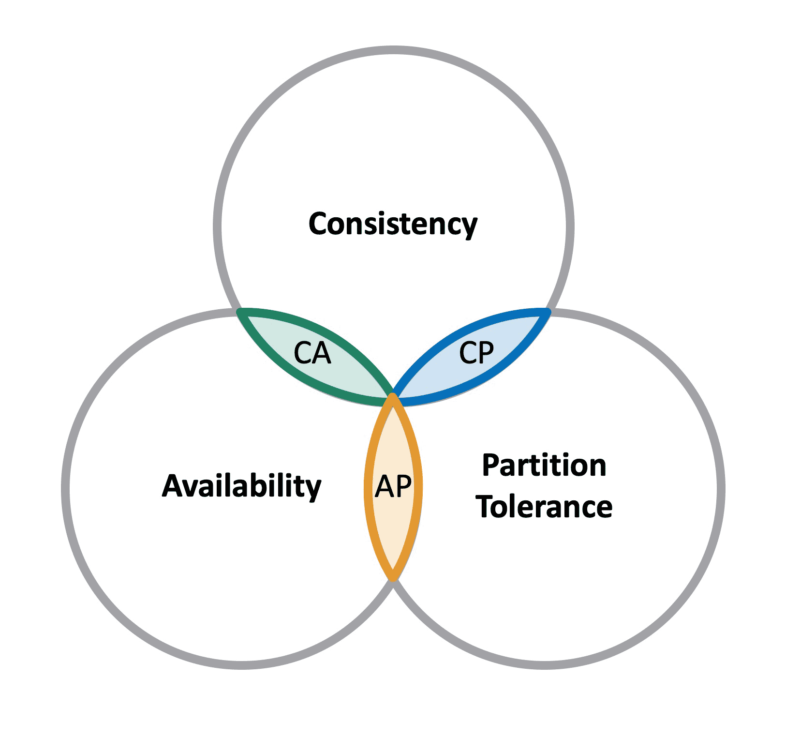
\includegraphics[scale=0.25]{/images/PNG/capTheorem}
\caption{CAP theorem diagram}
\label{fig:CAP}
\end{center}
\end{figure}
In order to guarantee the requirements of high availability, we decided to accept the cases in witch data shown to the user could be not up to date to the latest version in the database.

\section{Use cases}
\begin{figure}[H]
%\begin{center}
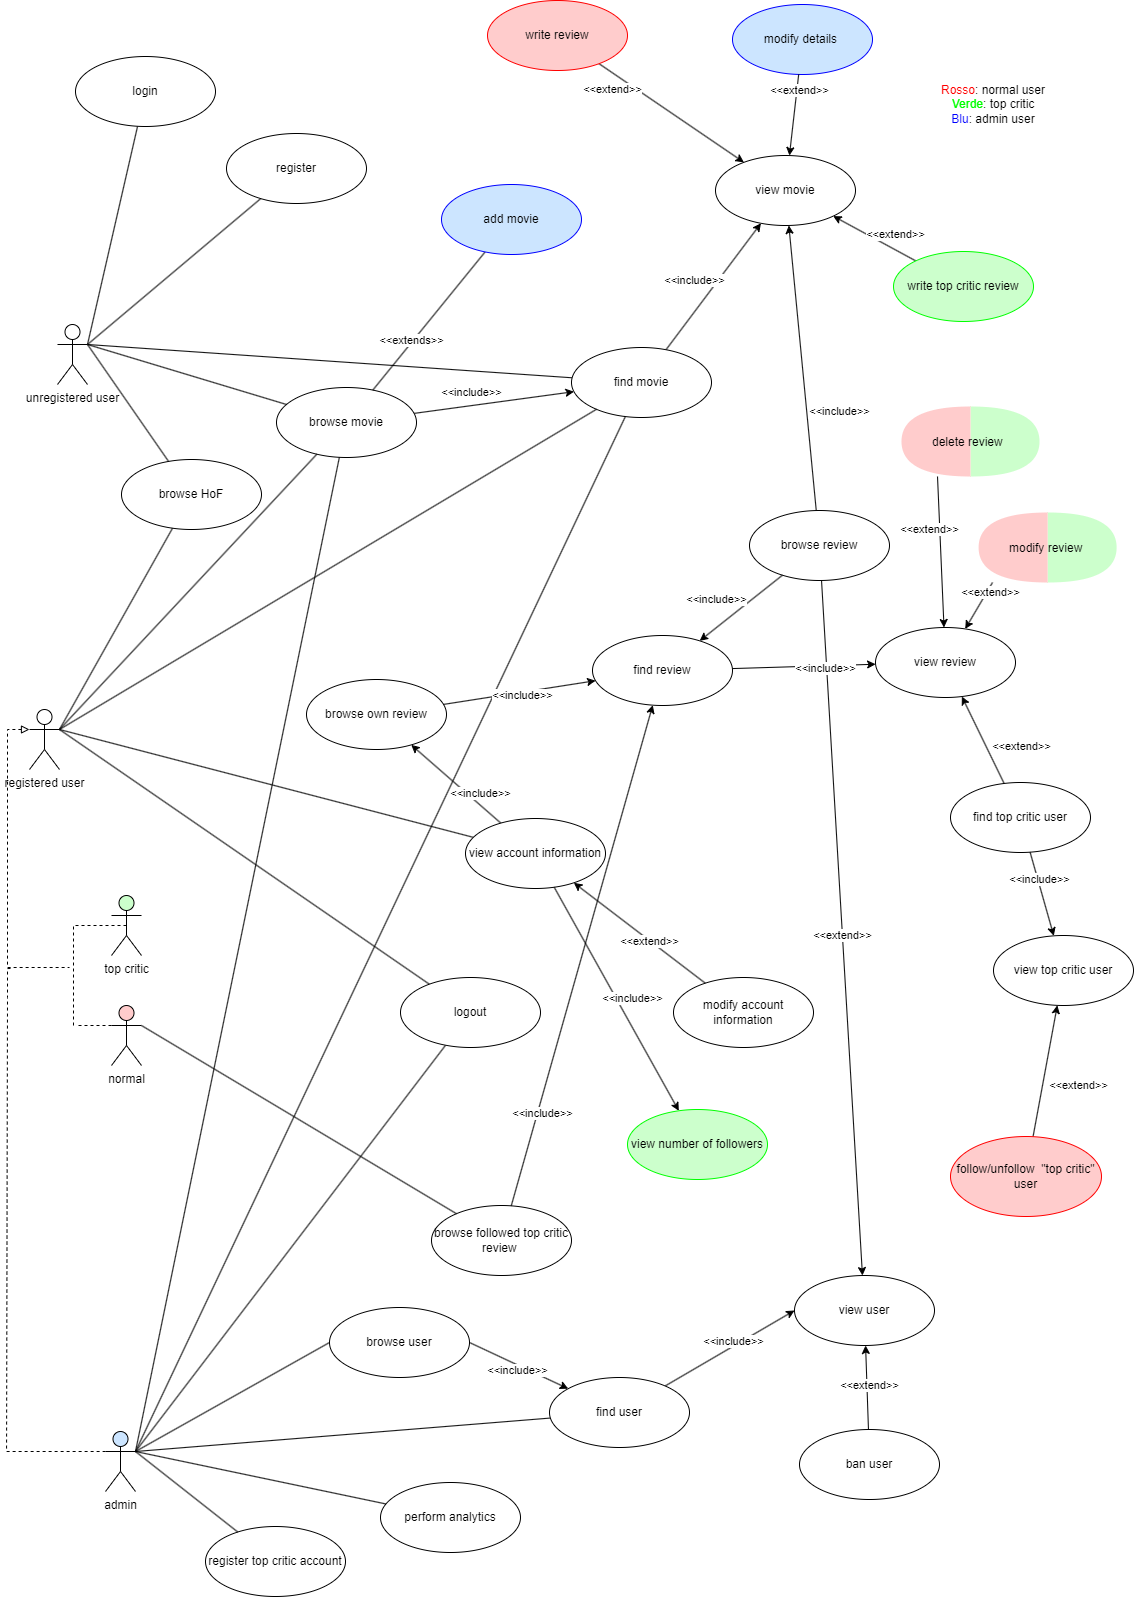
\includegraphics[scale=0.45]{/images/PNG/LatexUseCases}
\caption{Use cases}
\label{fig:UseCases}
%\end{center}
\end{figure}
The \emph{perform analytics} use case groups all of the following direct use cases:
\begin{itemize}
\item Group user base by age
\item Most active users and top critics
\item Most followed top critics
\end{itemize}

\section{Class analysis}
In this section we shall discuss the design of the various classes and how they relate to each other
\begin{figure}[H]
\begin{center}
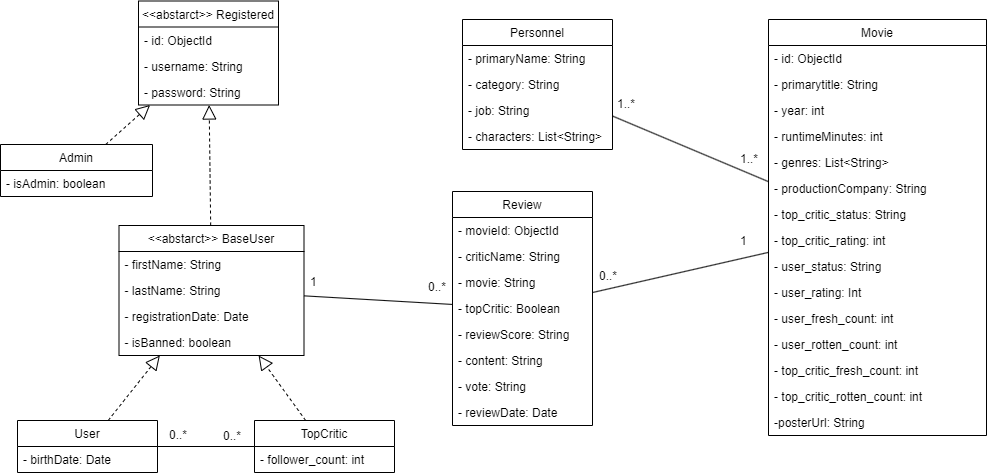
\includegraphics[scale=0.5]{/images/PNG/LatexClassDiagram}
\caption{Class Diagram}
\label{fig:UseCases}
\end{center}
\end{figure}
The diagram expresses the following relationships between the entities.
\begin{itemize}
	\item a BaseUser can write from zero to many reviews
	\item a Review can be written by a single BaseUser for a single Movie
	\item a Movie can have zero to many reviews and can have from 1 to many Personnel working in it
	\item a Personnel can work in 1 to many movies
\end{itemize}
%\end{document}